We have implemented a first prototype version of our approach in Matlab, relying on the Intlab~\cite{Ru99a} 
toolbox for computations with interval and affine arithmetic.
It allows us to first demonstrate in Section~\ref{sec:exp_bruss} the good behaviour of our inner-approximated flowpipes
 on the quite difficult Brusselator model. % plus des elements permettant de quantifier le cout de surapprox par rapport a sousapprox
Then, in Section~\ref{sec:exp_compar}, we provide some elements of comparisons to the experimental results 
given in the related work. 
 
\subsection{Brusselator}
\label{sec:exp_bruss}

We consider in this section the following instance of the Brusselator system, slightly different  from the version of  Example~\ref{running0}, but
which is the one studied in the related work:
$$\left\{\begin{array}{rcl}
\dot{x}_1 & = & 1+x_1^2x_2-2.5x_1 \\
\dot{x}_2 & = & 1.5x_1-x_1^2x_2
\end{array}\right.$$
\noindent with $x_1(0) \in [0.9,1]$ and $x_2(0) \in [0,0.1]$.

%\paragraph{Control of the wrapping effect}
We first use Taylor models of order 3 in time, which we first evaluate for inner and outer-approximations 
with plain interval arithmetic. When computing flowpipes for time ranging between $0$ and $1$, 
we see, in Figure~\ref{fig:brusselator_order3_t1}, that the width of the outer-approximation 
(external dashed lines) quickly increases, while the 
width of the inner-approximation (internal dotted lines) decreases even more quickly, 
until it disappears at time 0.6: after this time, the inner-approximation is empty. Indeed, it is well 
known that effective methods should be used to control this wrapping effect, for instance mean-value 
forms or matrix preconditioning. In our implementation, we control wrapping by using 
affine arithmetic to evaluate these models. %While accurate as shown in Figure \ref{fig:brusselator_order3_t1} (inner
%and outer approximations are solid lines), it will be more costly than using 
%a method specially optimized for these Taylor model. 
%\ForAuthors{Tu penses? Comme ca je n'en serais pas completement sur?}
%However, 
This is convenient for prototyping, 
as we rely on the implementation of affine arithmetic present in the Intlab 
toolbox.
 
\begin{figure}[htbp]
\begin{center}
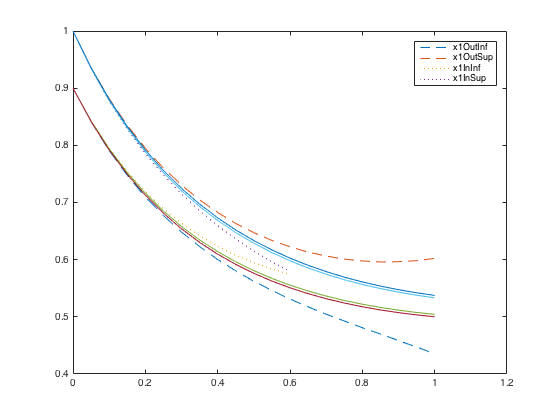
\epsfig{file=brusselator_x1_IA_AA.png,clip=,width=9cm}
\end{center}
\caption{Brusselator, evaluation of the Taylor models (order 3) with interval vs affine arithmetic \label{fig:brusselator_order3_t1}}
\end{figure}

In the following experiments, we use Taylor models of order 4, and represent respectively in Figures~\ref{fig:brusselator_order4_x1_t10} and~\ref{fig:brusselator_order4_x2_t10}, the inner and outer approximated flowpipes for variables $x1$ and $x2$, with an evaluation in affine arithmetic, up to a maximum time $t=10$. We see that for both variables, while the width of the outer-approximation stays relatively stable with time, the width of the inner-approximation can decrease until the inner-approximation becomes empty, but the width can still later be non-zero again. This is the case for instance on variable $x_2$ around time $t=4$. Also, we can note that the inner-approximations on x1 and x2 do not get empty at the same time. 
%At first look, this could appear as a bug in our implementation, but this is not the case. 
This is not a bug : this phenomenon is an illustration of the fact detailed in Section~\ref{practicalissues}, that when adding an improper with a proper interval, we can get a proper interval, which results in an empty inner-approximation, but this does not prevent us to keep computing the Taylor models that can give non-empty inner-approximations at later times, depending on the behaviour of the Jacobian of the flow.    

\begin{figure}[htbp]
\begin{center}
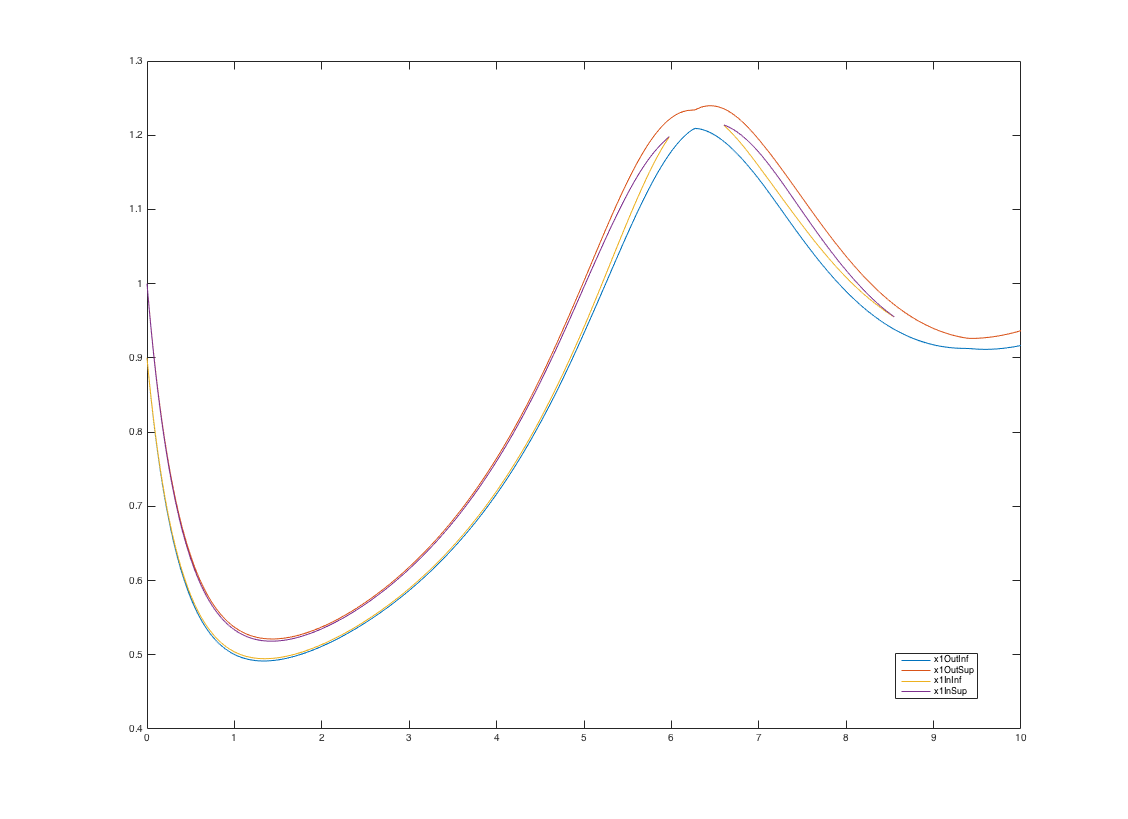
\epsfig{file=brusselator_x1_t10.png,clip=,width=9cm}
% ou version non commentée : 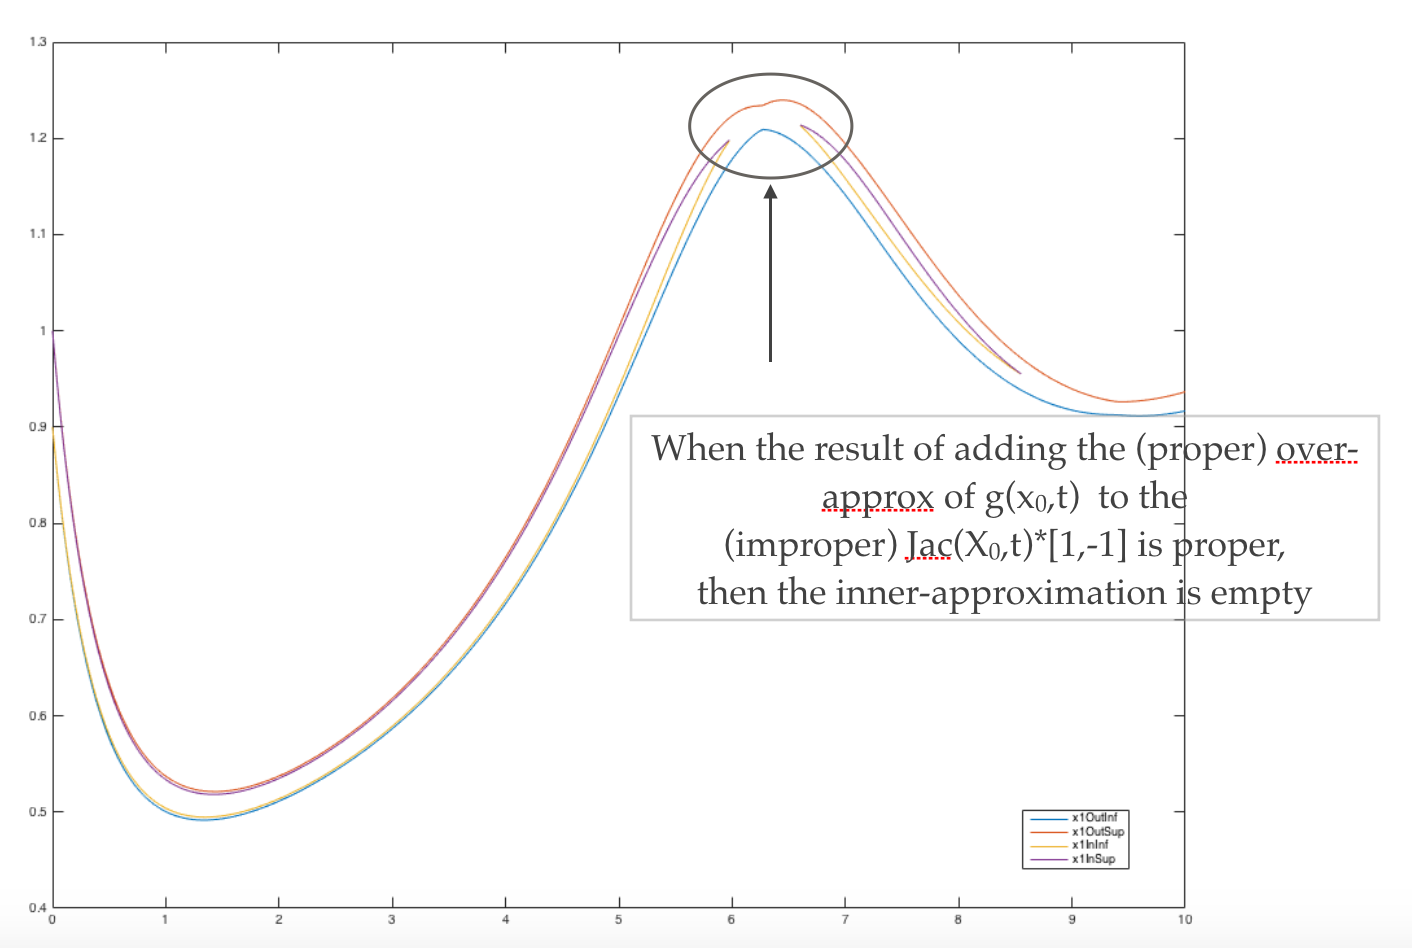
\epsfig{file=brusselator_x1_t10_comment.png,clip=,width=10cm}
\end{center}
\caption{Brusselator (x1), evaluation of the Taylor models (order 4) with affine arithmetic \label{fig:brusselator_order4_x1_t10}}
\end{figure}

\begin{figure}[htbp]
\begin{center}
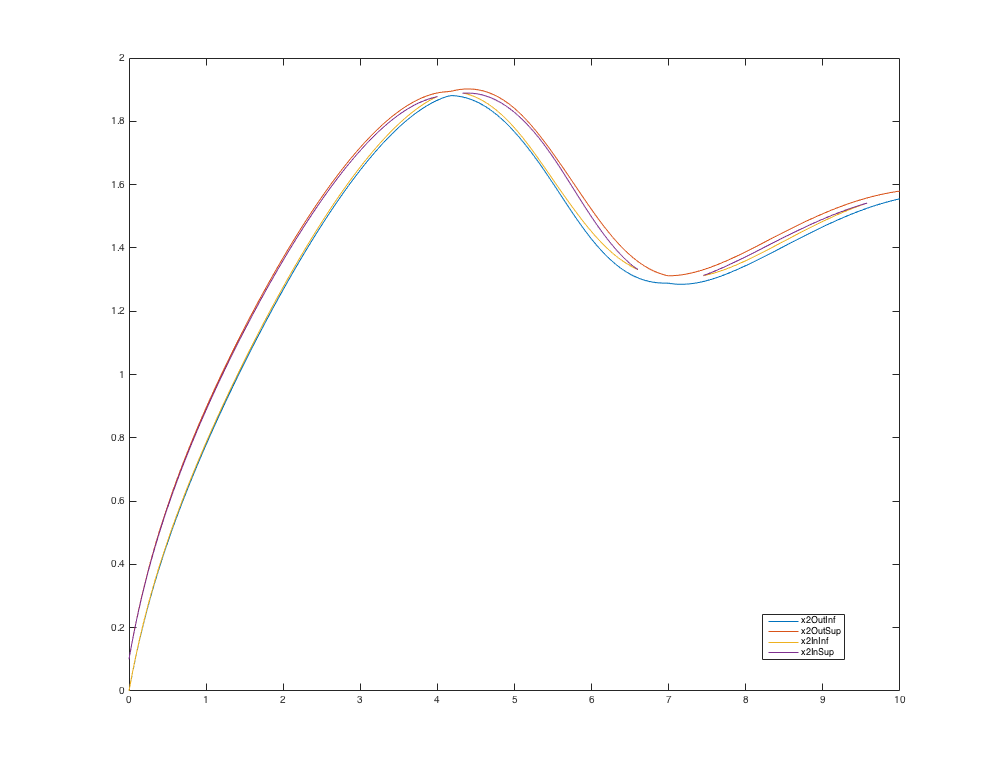
\epsfig{file=brusselator_x2_t10.png,clip=,width=9cm}
\end{center}
\caption{Brusselator (x2), evaluation of the Taylor models (order 4) with affine arithmetic \label{fig:brusselator_order4_x2_t10}}
\end{figure}


%------------------------------------------------------------------------------------------------------------------------------------------------

% Exemple retiré car je n'arrive pas a bioen le traiter pour le moment
%\subsection{Car on the hill}
%\[ \left\{ 
%\begin{array}{lll} \dot x_1 & = & x_2 \\
%\dot x_2 & = & - 9.81 \sin(\frac{dg}{dx}(x_1))-0.7 x_2 + u
%\end{array}
%\right.
%\]
%where \[ g(x) = \frac{1}{2} (-\frac{1.1}{1.2} \cos(x) + \frac{1.2}{1.1} cos(1.1x)), \]
%the command $u$ is bounded in $[-2,2]$, the initial condition is $x_1(0) \in [-1,1]$, $x_2(0) \in [-1,1]$, 
%and we have limit conditions $x_1(t) \in [-1,13]$, $x_2(t) \in \R$ (conditions as in T. Le Mezo's document ``viability list of problems'')

%\SP{Si on peut montrer qu'on peut soit reussir a remonter la cite soit rester bloque, un peu comme T. Le Mezo a montre dans sa pres a brest, ca serait chouette. 
%Mais au moins dans l'implem matlab ca explose completement, mais relativement bizarrement: je ne suis qu'a moitié confiante sur l'AA dedans ...}
%}

\subsection{Comparisons to the related work}
\label{sec:exp_compar}
We provide in this section some elements of comparisons to the experimental results given in the related work~\cite{Underapproxflowpipes,underapprox16}.
Let us highlight that it is difficult to have a fair comparison, as on the one hand, evaluating the compared accuracy of these methods is difficult, 
and on the other hand we only used a very basic Matlab implementation of our approach, whereas the related work relies on actual implementations,
using optimized solvers such as VNode. In order to partially account for this overhead of our preliminary implementation, we will also compare in our experiments 
the computation time of our inner (and outer-) approximated flowpipes, with the time taken by our implementation for the classical outer-approximation 
of Taylor model flowpipes. 

%\ForAuthors{J'aime bien l'idee de comparer le cout du calcul sous-approx
%a celui de l'outer-approx du meme degre avec ton implem - tu le mets en
%remarque plus loin. Je pense qu'il faut l'expliquer un peu ici?
%Ok je ferai quand j'aurai integre ces resultats}

Among the examples studied in both ~\cite{Underapproxflowpipes} and \cite{underapprox16}, we first selected
the version of the Brusselator introduced in section~\ref{sec:exp_bruss} as a representative of the systems of low degree. 
We chose as second example the following biological system, because of its higher degree (7), to investigate the way our approach scales. 
\begin{equation}
\dot{\left(\begin{array}{c}
x_1 \\
x_2 \\
x_3 \\
x_4 \\
x_5 \\
x_6 \\
x_7
\end{array}\right)} = \left(\begin{array}{c}
-0.4x_1+ a x_3x_4 \\
0.4x_1-x_2 \\
x_2- a x_3x_4 \\
a x_5x_6- a x_3x_4 \\
- a x_5x_6+ a x_3x_4 \\
0.5x_7- a x_5x_6 \\
-0.5x_7+ a x_5x_6
\end{array}\right)
\end{equation}
In this system, $a$ is a parameter which is taken, from our understanding, equal to 50 in \cite{Underapproxflowpipes} and to 5 in \cite{underapprox16}. 
We will use the corresponding value of the parameter when comparing to the realted work.

\subsubsection{Comparison to \cite{Underapproxflowpipes}}
In  \cite{Underapproxflowpipes}, the  accuracy of computations is measured by the minimum width ratio 
\[ \gamma_{\min}=\min{\frac{\gamma_u(v)}{\gamma_o(v)}}, v \in V \]
where $V$ is a set of vectors, and $\gamma_u(v)$ and $\gamma_o(v)$ measure respectively the width of the inner-approximation and outer-approximation
in direction $v \in V$. 
Intuitively, the larger this ratio, the better the approximation. 
Our method naturally gives inner ranges for the projection of the flow system on its state variables (although we can also directly deduce from our Taylor models 
an inner-approximation of the range of any linear function of these variables, and also define a joint range, as 
already mentioned).
%\ForAuthors{Deja dit avant, on insiste ou pas?} 
We thus measure in our case \[ \gamma_{\min}=\min_{i}{\frac{\gamma_u(x_i)}{\gamma_o(x_i)}}, \]
where the $x_i$ are the state variables of the system. We believe this corresponds to the measure that was used for experiments 
in~\cite{Underapproxflowpipes}, as they mention that the vectors are selected along the dimensions (axis-aligned).

%\ForAuthors{Sriram dit dans le dernier paragraph ``Results'' de [1], 
%pour $\gamma_{min}$ que ``The vectors are selected along the dimensions
%(axis-aligned).''? Donc ca serait comparable a nous?}
\paragraph{Comparison on the Brusselator}
We first consider the Brusselator system, with an initial set taken in~\cite{Underapproxflowpipes}, defined by 
$x_1 \geq 0.9$, $x_2 \geq 0$, $x_1+x_2-1 \leq 0$, which we can project on $1 \geq x_1 \geq 0.9$, $0.1 \geq x_2 \geq 0$.
Naturally, this outer-approximation of the initial set is quite inaccurate, which will result in a lower quality of the inner-approximation
that must be taken into account in the comparison to the results of~\cite{Underapproxflowpipes}. In our approach, 
we can actually consider initial sets that are not given as intervals, for instance given as zonotopes 
(in the present case, we could use a zonotopic outer-approximation of the simplex),  
but we did not investigate this here. 

%\ForAuthors{Evidemment, la on peut perdre pas mal de precision par rapport
%a Sriram vu qu'on prendre le carre englobant le triangle en condition initiale. Ptet insister la dessus?}
%\ForAuthors{On peut le dire - je l'ajoute - mais en meme temps c'est notre faute si on n'est pas capable 
%de prendre en compte ce genre de conditions initiales ;) Certes mais selon
%la methode ensembliste utilisee pour abstraire les coefficients de Taylor
%(dont $z_0$) on peut faire des choses plus ou moins elaborees. On pourrait
%faire une approximation zonotope du triangle (pas commode neanmoins) et
%faire mieux eventuellement. En tout cas on pourrait dire que l'on n'est pas
%limite forcement a des intervalles en entree?}
In ~\cite{Underapproxflowpipes}, the authors study the result for T = 3 and T = 4. We choose, as they do, 4th order Taylor models, 
but take a larger time step $h=0.05$ in order to keep comparable (though much larger here) analysis time. In this case, our implementation until $T=4$
takes a total of 776 seconds (to compute both outer and inner approximations), where \cite{Underapproxflowpipes} takes 89 seconds.
Our implementation is thus almost an order of magnitude larger, however we believe this is very much due to our naive implementation 
with matlab and the affine arithmetic of Intlab. This can be for instance quantified by measuring the time  that our implementation of the classical 
outer-approximated Taylor Model takes on the same example with the same parameters: it takes here 213 seconds, so that the overhead due to inner-approximation 
is really of the same order of magnitude (intuitively, the time from outer to inner-approximation with our approach should indeed approximately 
be multiplied by the dimension of the Jacobian). 
\ForAuthors{Pas hyper hyper clair? Sinon je peux aussi te dire combien VNODE prend de temps pour la outer-approx, ca donne aussi une idee du facteur du a l'implem?}
% Our implementation takes a total of 3400 secs (for computing both outer and inner approximations). pour 0.02

%\begin{center}
%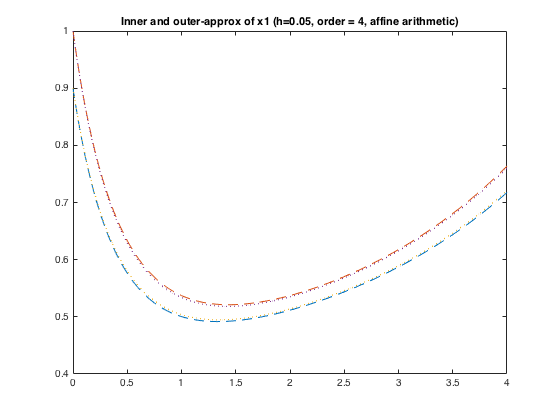
\epsfig{file=sriram_bruss_order4_t4_x1.png,clip=,width=8cm}
%\end{center}
%\begin{center}
%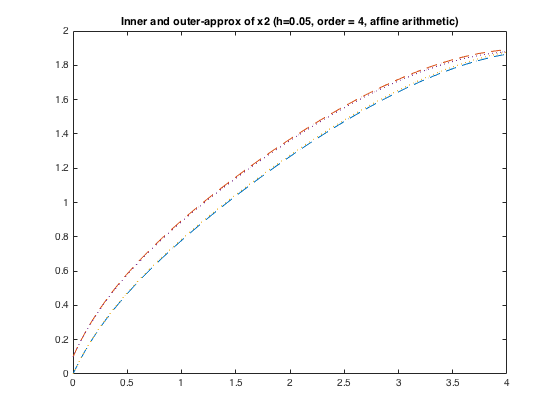
\epsfig{file=sriram_bruss_order4_t4_x2.png,clip=,width=8cm}
%\end{center}
\begin{figure}
\begin{tabular}{cc}
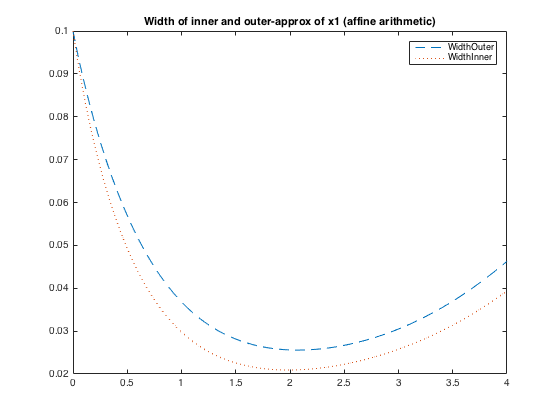
\epsfig{file=sriram_bruss_order4_t4_widthx1.png,clip=,width=4.cm}
&
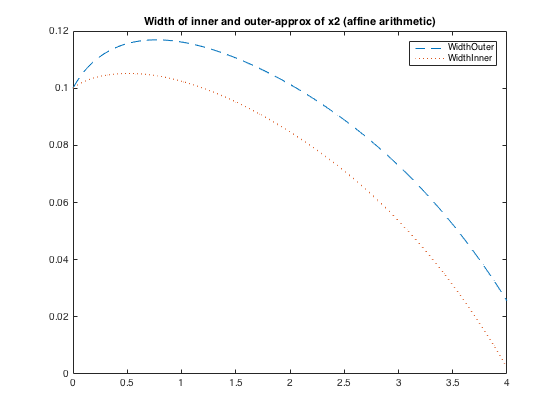
\epsfig{file=sriram_bruss_order4_t4_widthx2.png,clip=,width=4.cm}
\end{tabular}
\caption{Width of the inner- and outer-approximations of x1 and x2 with time (order 4, h=0.02)}
\ForAuthors{Trop petit comme ca?}
\end{figure}

\begin{figure}
\begin{center}
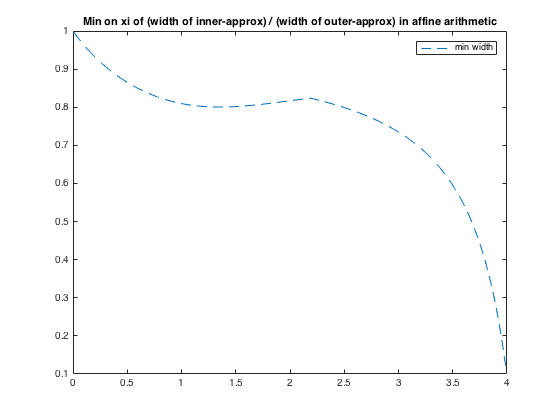
\epsfig{file=sriram_bruss_order4_t4_minwidth.png,clip=,width=8cm}
\end{center}
\caption{Evolution of $\gamma_{\min}$ with time}
\label{ex:width_sriram_bruss}
\end{figure}
On Figure~\ref{ex:width_sriram_bruss}, we see that at $t=3$, the relative width of the inner-approximation over the
outer-approximation is of order $0.7$, which is equal to the value given in Table~1 of \cite{Underapproxflowpipes}. 
However, this ration decreases quickly, mostly due to the $x_2$ component, and at $t=4$, we get a ratio very close to $0.1$,
instead of 0.55 as in [1]. Indeed, $t=4$ is a time at which, as already seen in Section~\ref{sec:exp_bruss}, our 
inner-approximation of variable $x_2$ is temporarily of lower quality. 
We thus get on this example, with the same parameters for the Taylor models, worse inner-approximation quality for a longer time of our implementation. 
However, our approach allows us here to reduce the order of our models and take larger time steps for very close quality of results on $\gamma$: taking order 3 
Taylor models and a timestep of 0.1, we get a computation time of 93 seconds, thus comparable now to \cite{Underapproxflowpipes}. 
Further decreasing the precision starts degrading the quality of results.    

%\ForAuthors{Mais je crois quand meme que de ne
%pas demarrer par un simplex doit pouvoir changer pas mal! Je peux essayer
%de demander a Xin Chen si on peut facilement avoir leur resultat sur le
%carre initial, pour T=3 et T=4? Peut-etre aussi essayer l'ordre 5 de notre
%cote? J'aurais presque compare le width de under-approx a l'ordre 5 sur
%l'over-approx a l'ordre 4, on a un peu l'impression qu'on ``perd'' un ordre
%dans la sous-approx.}

%\ForAuthors{Oui ordre 5 je voulais le faire c'etait prevu mais comme c'est long a calculer j'ai pas eu le temps vendredi;
%et je suis d'accord pour l'ordre car en fait ce que je calcule actuellement c'est il me semble des TM a l'ordre 3 
%sur la jacobienne - car j'ai pour cela besoin des coeff des TM a l'ordre 4 des TM sur le flot. Si ca marche bien a l'ordre 5 je raconterai ca - evidemment ca va etre encore plus couteux ... 

%Dans tous les cas, comparer le temps sur et sous
%approx, ca permet de donner un facteur pour le temps, du essentiellement
%a l'implem.}


%order 5 (4 in the Jacobian), h = 0.05 2168 sec 
%h=0.02, 4684 sec for inner/outer-approx  - 12461 si je ne diminue pas les dependances a chaque pas

%[en gardant les relations] order 4 h = 0.05 outer-approx only 213 sec, order 4 h = 0.05 outer-approx and inner-approx 776
%[meme chose sans garder les relations]  outer-approx only 120 sec  outer-approx and inner-approx 451 precision un peu moindre

%\ForAuthors{Add elements allowing to compare the cost of inner-approx comapred to over-approx of same degree: where to put this and on which example, see later}  
\paragraph{Comparison on the biological system}
We now consider the biological system, with initial condition $\x_0 \in [0.1,0.1175] \times...\times [0.1,0.1175]$, which is an outer-approximation
of the simplex taken in  \cite{Underapproxflowpipes}, and we compute inner and outer approximated flowpipes for time in [0,0.2], 
with order 3 Taylor Models and a stepsize of 0.02. The computation completes in 118 seconds, and we get as a measure of quality of the approximation 
$\gamma(t=0.2) \approx 0.61$, which is this time much better than the $\gamma(t=0.2) = .25$ obtained in 632 seconds in  \cite{Underapproxflowpipes}, 
in spite of using a larger step size of 0.02 (0.002 in \cite{Underapproxflowpipes}). This seems to confirm that our approaches scales very well to high dimensional systems. 
Again, the 118 seconds for the inner-approximation flowpipe must also be compared to the 36.9 seconds that our implementation of the classical 
outer-approximated Taylor Model takes with the same parameters.

We also measure as an indication of the accuracy the mean value on the components $x_i$ of the distance between the inner and outer approximations, $\sum_i=1^n \frac{|x_i^{out} - x_i^{in}|}{n}$,
which is an over-estimation of the error between our inner-approximation and the exact reachable state: this value for $T=0.2$ is $4.10^{-3}$.

%elapsed_time_AA =  122.1330, step = 0.02, order 3
%elapsed_time_surapprox_AA =  39.6906


% je l'enleve pas passionnant 
%\begin{figure}
%\begin{center}
%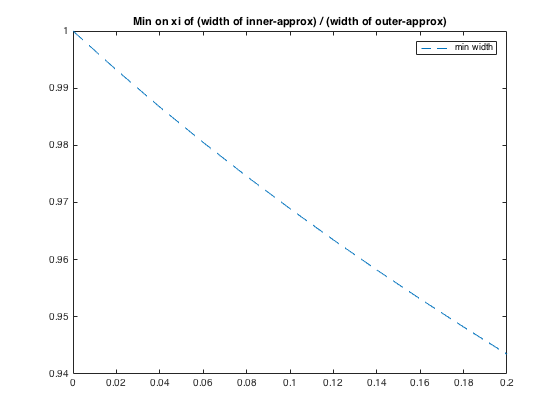
\epsfig{file=biological_sriram_002_order2_width.png,clip=,width=8cm}
%\end{center}
%\caption{Evolution of $\gamma_{\min}$ with time on the biological system}
%\label{ex:width_sriram_bio}
%\end{figure}

\subsubsection{Comparison to \cite{underapprox16}}
\paragraph{Comparison to \cite{underapprox16} on the Brusselator}
In \cite{underapprox16} the authors take $X=[0.3, 0.4] \times [0.5, 0.7]$ for a time frame in [0,1.1], and a time step h=0.05. 
We compute the inner and outer-approximations, with order 3 Taylor Models, evaluated in affine arithmetic, in 45 seconds.
In comparison, our implementation of the classical outer-approximated Taylor models takes 16 seconds. 
%In Figure~\ref{fig:bruss_cav16}, we represent the inner and outer-approximations obtained for $x_1$ and $x_2$.  
%\begin{figure}[htbp]
%\begin{tabular}{cc}
%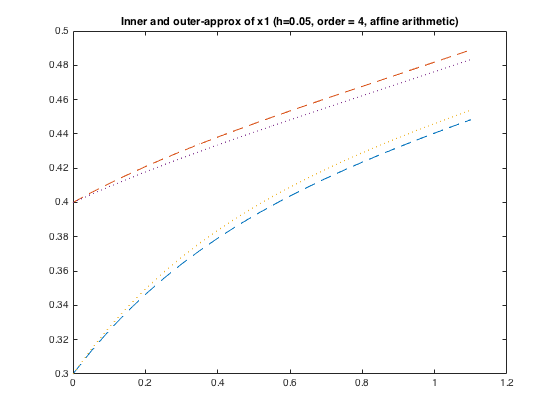
\epsfig{file=cav16_bruss_order4_x1.png,clip=,width=4cm}
%&
%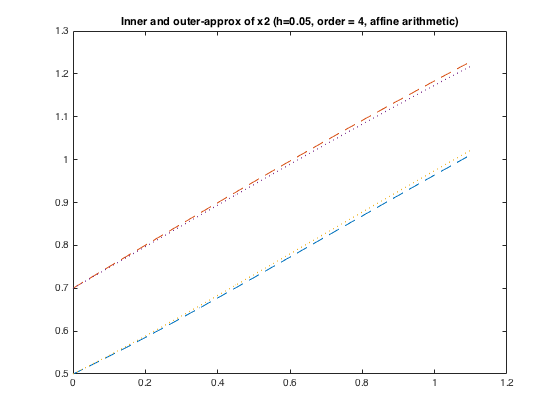
\epsfig{file=cav16_bruss_order4_x2.png,clip=,width=4cm}
%\end{tabular}
%\caption{Inner and outer approximations (order 4) for $x_1$ and $x_2$ \label{fig:bruss_cav16}}
%\ForAuthors{Trop petit?}
%\end{figure}
In Figure~\ref{fig:bruss_cav16_dist}, we represent the maximum distance between the inner 
and the outer approximations, for each variable $x_1$ and $x_2$.
\begin{figure}[htbp]
\begin{center}
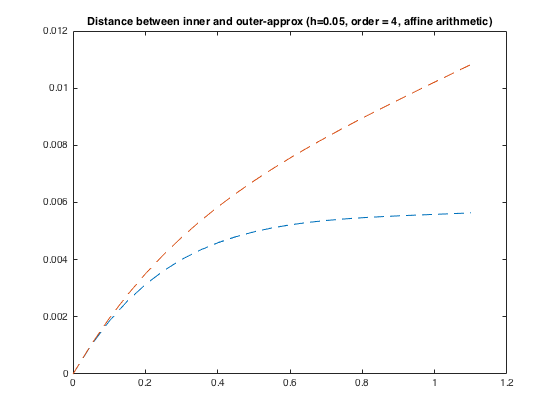
\epsfig{file=cav16_bruss_order4_distance.png,clip=,width=8cm}
\end{center}
\caption{Maximum distance between the inner and outer approximations for x1 and x2 \label{fig:bruss_cav16_dist}}
\end{figure}
This distance should in some sense be comparable to the parameter  $\epsilon_M$ which is used to estimate the precision in \cite{underapprox16}.
We find a distance equal to 0.005 for $x_1$, and 0.01 for $x_2$, which is 10 times larger than their estimation of 0.001, in 55 seconds, 
of the parameter  $\epsilon_M$ used to estimate the precision in \cite{underapprox16}, which we beleive comparable in spirit to our distance. 

\ForAuthors{Eric. Commenter sur ce que veut dire leur epsilonM }

%\ForAuthors{De ce que je comprends, leur $\epsilon_M$ est la pr\'ecision
%avec laquelle ils donnent une surapprox de la frontiere du reachable set.
%Leur precision c'est la taille (en chaque coordonnee) des boites qui 
%font cette surapprox. Donc au pire ils sont a $\epsilon_M$ de la frontiere,
%dans cette collection de boites, dans chaque direction. Apres ils trouvent
%un polytope maximal \`a l'interieur de cette approximation de frontiere
%par collection de boites. Donc ben difficile a comparer...Par rapport
%au vrai reachable set ils seront en general plus ou moins a $\epsilon_M$
%de la, mais peut-etre bcp plus, peut-etre bcp moins s'ils ont de la chance...
%Eux ils font avec $\epsilon_M=0.001$ et $\epsilon_M=0.0002$ ; je n'ai 
%pas trouve a quel ordre ils utilisent VNODE (j'ai souvenir d'un ordre
%20 que je ne trouve plus?). La a cause du $x_1$ pour une fois, on est
%en gros potentiellement 10 fois moins bons, mais il y a aussi la distance
%de la surapprox au vrai reachable set. On pourrait aussi utiliser un 
%modele de Taylor surapprox (voire VNODE?) a ordre bcp plus eleve pour
%affiner cette distance? Ou alors integrer le brusselator, numeriquement
%au hasard sur pas mal d'etats initiaux et voir la distance? (un peu comme
%eux avec leurs simus RK4?). On peut essayer aussi au moins a l'ordre 5
%voir si on ameliore cette distance? Eux meme avec VNODE, ils mettent
%55s pour le premier $\epsilon_M$ et 410s pour le deuxieme, on devrait
%pouvoir se comparer agreablement vu qu'on a du Matlab, et plein de choses
%non optimisees?}

\paragraph{Comparison on the biological system}
We now consider the biological system, with, as in \cite{underapprox16}, initial condition $\x_0 \in [0.1,0.1175] \times...\times [0.1,0.1175]$, 
and to compare our results to their backward estimate, we compute inner and outer approximated flowpipes on the reverse flow, 
for time in [0,0.2] , and use order 3 Taylor Models and a stepsize of 0.02.

We get as width of inner-approximation on each component at time 0.2 the following :

\begin{tabular}{l|c|c|c}
 & õur inner/outer & VNODE (order 20) &  inner\cite{underapprox16} \\
Time & 115sec (36 for outer-approx only) & < 1 sec & 0.67 sec \\
$x_1$ &  [  -0.016286,   0.0010362] / [  -0.016547,   0.0012979] & [-0.0166, 0.00131] & [-0.0152,0.000] 

\end{tabular}

 $[   -0.01628,    0.00104]\times[   -0.01834,    0.00256]\times [   -0.01515,    0.00417]\times 
[   -0.01489,    0.00088] \times[   -0.01488,    0.00089]\times[   -0.0150,    0.00248]\times [   -0.01661,    0.00106]$

$[  -0.01628536833380,   0.00103619844301]  [  -0.01833708041159,   0.00255842760143]  [  -0.01514208680158,   0.00416990950253]  [  -0.01488096912574,   0.00087696255375] 
[  -0.01487744391170,   0.00088145048369]  [  -0.01492448895828,   0.00247920964913]  [  -0.01660493465136,   0.00105021396051] $

to be compared to the $[-0.0152,0.000]\times[-0.0169,0.0011]\times [-0.00140,0.0030]\times[-0.0141,0.0001]\times [-0.0141,0.0001]\times [-0.0138,0.0014]\times [-0.0155,0.0000]$
of \cite{underapprox16} .

With VNODE at order 20 (with an execution time smaller than 1 second, which confirms the poor efficiency of our matlab implementation...) 
$[-0.0166, 0.00131]
[-0.0184, 0.00262]
[-0.0154, 0.00451]
[-0.0154, 0.00141]
[-0.0154, 0.00141]
[-0.0152, 0.00277]
[-0.0169, 0.00131]$

Our outer-approximation is $ [  -0.01654701249765,   0.00129784260686]  [  -0.01834542409233,   0.00256677128217]  [  -0.01540563322262,   0.00443345592357]
[  -0.01539838418560,   0.00139437761361] [  -0.01538981256285,   0.00139381913484] [  -0.01519231394425,   0.00274703463510] [  -0.01686300688068,   0.00130828618983]$
which look tighter than the VNODE order 20 results (???). 

The mean distance from our inner-approximation to our outer-approximation, defined by $\sum_i=1^n \frac{|x_i^{out} - x_i^{in}|}{n}$, is thus equal to $4.10^{-4}$ 
when the mean distance from the inner-approximation of \cite{underapprox16} to our approximation is $2.10^{-3}$ 

%\ForAuthors{A comparer au related workj, mais width de am surapporx (a recopier) < width de leur surapprox sur certains cas => wierd}

% [t,y] = ode23(@Bio_forode,[0 0.2],[-0.015; -0.015 ; -0.015; -0.015; -0.015; -0.015; -0.015]); => x3 sort de leur boite

%\paragraph{Comparaison to \cite{Underapproxflowpipes} on the biological system}

%for time in $[0,0.2]$, but again on differential initial conditions. 



\subsection{Other examples}
%\paragraph{Moore-Greitzer model of a jet engine}
%\begin{equation}
%\dot{\left(\begin{array}{c}
%x \\
%y
%\end{array}\right)} = \left(\begin{array}{c}
%-y-1.5x^2-0.5x^3-0.5 \\
%3x-y
%\end{array}\right)
%\end{equation}
%The initial set is given by the simplex 
%$$X_0=\{(x,y) \in \R^2 | -x \leq -0.9 \wedge -y \leq -0.9\wedge x+y-2 \leq 0\}$$

%In \cite{Underapproxflowpipes}, two cases are considered : 
%\begin{itemize}
%\item computation of the inner and outer approximations of the reachable set at time
%$t=0.04$
%\item computation of the inner and outer approximations of the reachable set at times
%in [0,3] (using a step-size $\delta=0.02$)
%\end{itemize}

%\ForAuthors{Je rajoute les equations plus tard}

%\paragraph{Shimizu-Morioka}

%\paragraph{Steam governor}

%\paragraph{R\"ossler}


%\paragraph{Lorenz}

%\paragraph{Lotka-Volterra}
%(also from \cite{underapprox16}?)

%\begin{equation}
%\dot{\left(\begin{array}{c}
%x_1 \\
%x_2 \\
%x_3
%\end{array}\right)} = \left(\begin{array}{c}
%x_1x_2-x_1x_3 \\
%x_2x_3-x_2x_1 \\
%x_3x_1-x_3x_2
%\end{array}\right)
%\end{equation}

%\paragraph{Coupled Van der Pol}

%The next set of examples is taken from \cite{underapprox16}. 

%\paragraph{Electromechanical oscillation}

%\begin{equation}
%\dot{\left(\begin{array}{c}
%x \\
%y
%\end{array}\right)} = \left(\begin{array}{c}
%y \\
%0.2-0.7sin(x)-0.05y
%\end{array}\right)
%\end{equation}
%The initial set is given by $[-0.1,0.1]\times [2.9,3.1]$. We are looking at an 
%inner-approximation at times $t=0.5$ and $t=3$. 

%\paragraph{Van der Pol}

%\begin{equation}
%\dot{\left(\begin{array}{c}
%x_1 \\
%x_2
%\end{array}\right)} = \left(\begin{array}{c}
%x_2 \\
%-0.2(x^2_1-1)x_2-x_1
%\end{array}\right)
%\end{equation}

\paragraph{Integrable systems}
To make precision estimates of our method. 

%$$\dot{u}=u^2$$
%\noindent with $u(0)=u_0$. 
%Then $u=\frac{u_0}{1-u_0t}$

The logistic equation :

$$\dot{u}=\lambda u(1-u)$$
\noindent with $u(0)=u_0$. Then
$u(t)=\frac{u_0e^{\lambda t}}{1-u_0+u_0e^{\lambda t}}$.

\ForAuthors{Pour $0 < u_0 < 1$ et $\lambda > 0$ par exemple, c'est une fonction decroissante
en $u_0$ et $\lambda$ donc on trouve facilement les bornes!}

%\ForAuthors{Pas mal d'autres dans \url{http://www.math.umn.edu/~olver/am_/odz.pdf} mais les deux au dessus paraissent simples et raisonnables, surtout la 
%logistic equation?}

%$$\dot{y} = \frac{a}{\sqrt{y}}+y$$
%\noindent with $y(a)=1$
%Solution is :
%$$y(t)=\left(exp\left(\frac{3t}{2} - \frac{3a}{2} + log(a + 1)\right) - a\right)^{\frac{2}{3}}$$
%(from Mathworks - can find $y(0)$ and translate it into polynomial system?)

\subsection{Conclusion}
Resultats preliminaires qui peuvent ne pas sembler que positif mais a priori essentiellement dus a la presente implem
\ForAuthors{
- comparaison sur / sous-approx => sous-approx competitive en complexite par rapport aux modeles de Taylor classiques\\
- bon passage a l'echelle sur degre 7 ? \\
- IA / AA laissant etendre que implem AA utilisee tres sous-optimale
- un des interets est qu'on peut raffiner la precision (sur et sous-approximee) en montant en ordre a la demande, du style algo a pas ou ordre adaptatif par cette 
estimation directe de l'erreur!
}
